\documentclass[]{elsarticle} %review=doublespace preprint=single 5p=2 column
%%% Begin My package additions %%%%%%%%%%%%%%%%%%%
\usepackage[hyphens]{url}



\usepackage{lineno} % add
\providecommand{\tightlist}{%
  \setlength{\itemsep}{0pt}\setlength{\parskip}{0pt}}

\usepackage{graphicx}
\usepackage{booktabs} % book-quality tables
%%%%%%%%%%%%%%%% end my additions to header

\usepackage[T1]{fontenc}
\usepackage{lmodern}
\usepackage{amssymb,amsmath}
\usepackage{ifxetex,ifluatex}
\usepackage{fixltx2e} % provides \textsubscript
% use upquote if available, for straight quotes in verbatim environments
\IfFileExists{upquote.sty}{\usepackage{upquote}}{}
\ifnum 0\ifxetex 1\fi\ifluatex 1\fi=0 % if pdftex
  \usepackage[utf8]{inputenc}
\else % if luatex or xelatex
  \usepackage{fontspec}
  \ifxetex
    \usepackage{xltxtra,xunicode}
  \fi
  \defaultfontfeatures{Mapping=tex-text,Scale=MatchLowercase}
  \newcommand{\euro}{€}
\fi
% use microtype if available
\IfFileExists{microtype.sty}{\usepackage{microtype}}{}
\bibliographystyle{elsarticle-harv}
\usepackage{longtable}
\usepackage{graphicx}
\ifxetex
  \usepackage[setpagesize=false, % page size defined by xetex
              unicode=false, % unicode breaks when used with xetex
              xetex]{hyperref}
\else
  \usepackage[unicode=true]{hyperref}
\fi
\hypersetup{breaklinks=true,
            bookmarks=true,
            pdfauthor={},
            pdftitle={Wiring between close nodes in biological networks evolves more quickly than between distant nodes},
            colorlinks=false,
            urlcolor=blue,
            linkcolor=magenta,
            pdfborder={0 0 0}}
\urlstyle{same}  % don't use monospace font for urls

\setcounter{secnumdepth}{5}
% Pandoc toggle for numbering sections (defaults to be off)

% Pandoc citation processing

% Pandoc header



\begin{document}
\begin{frontmatter}

  \title{Wiring between close nodes in biological networks evolves more quickly than between distant nodes}
    \author[Stony Brook University]{Alejandro Gil-Gomez}
   \ead{alejandro.gilgomez@stonybrook.edu} 
    \author[Stony Brook University]{Joshua Rest}
   \ead{joshua.rest@stonybrook.edu} 
      \address[Stony Brook University]{Department of Ecology \& Evolution, Stony Brook University, 650 Life Sciences Building, Stony Brook, NY 11794-5245}
    
  \begin{abstract}
  Lorem ipsum dolor sit amet, consectetur adipiscing elit. Curabitur eget porta erat. Morbi consectetur est vel gravida pretium. Suspendisse ut dui eu ante cursus gravida non sed sem. Nullam sapien tellus, commodo id velit id, eleifend volutpat quam. Phasellus mauris velit, dapibus finibus elementum vel, pulvinar non tellus. Nunc pellentesque pretium diam, quis maximus dolor faucibus id. Nunc convallis sodales ante, ut ullamcorper est egestas vitae. Nam sit amet enim ultrices, ultrices elit pulvinar, volutpat risus.
  \end{abstract}
   \begin{keyword} network biology, interactome, network evolution, phylogenetic comparative methods, drug-drug interactions\end{keyword}
 \end{frontmatter}

\hypertarget{introduction}{%
\section{Introduction}\label{introduction}}

Biological networks are representations of molecular interactions in the cell. The networks are constructed by collecting biochemical and genetic interactions between different kinds of biological entities, an approach that has improved drastically in the last decades with the advent of modern high-throughput methods. However, there are still many limitations for the gathering and analysis of biological networks, especifically for modelling network evolution across and within species. This is because many biological networks have poor quality or are incomplete, and because the number of organisms for which network data is available is still very limited (Jin et al. 2013; Cusick et al. 2005; Ghadie, Coulombe-Huntington, and Xia 2018). Despite these limitations, many advances have been made in characterizing static networks, and in developing a theoretical framework for studying their evolution across species.

Biological networks evolve as nodes and edges are added or lost. Nodes are added or lost as a result of different processes such as gene duplication, gene loss, pseudogenization, HGT or WGD (Wagner 2003; Cork and Purugganan 2004), while edges are modified as a result of non-synonymous substitutions in the nodes that affect the function of the node (i.e.~binding a protein domain, regulating gene expression, carrying out a metabolic or signaling process, etc) (Jensen 1976; Ghadie, Coulombe-Huntington, and Xia 2018). These events generate new random connections between nodes in the network, although not all motifs are equally abundant in biological networks (Picard et al. 2008), which have been proposed to be a result of natural selection removing deleterious connections and favoring advantageous ones (Picard et al. 2008). In addition, it has been shown that rewiring rates vary depending on the type of network being faster in regulation than metabolic networks (Shou et al. 2011). Specifically the relative rewiring rates for different types of networks are as follows: transcription factor regulatory networks \textgreater{} genetic interaction networks\textgreater protein interaction networks \textgreater{} metabolic pathway networks. In addition, rewiring rates also vary across network modules or between nodes depending on their role in the cell, their essentiality and possibly other factors. Previous studies have shown that there is an inverse relationship between highly connected proteins and their sequence conservation (Fraser et al. 2002), possibly due to strong purifying selection acting on interfacial sites (Zotenko et al. 2008). Despite these advances at studying the connections of individual nodes and global network rewiring rates, other metrics of inter-node connectivity remained unexplored, how quantitative differences between networks accumulate as a function of species divergence, and what role different inter-node network measures have on estimating the evolutionary rates of inter-node connectivity. For example, minimum distance between nodes, average node degree, and k-edge connectivity. In this paper, we use drug-drug interactions (DDIs) as a quantitative proxy measurement of inter-node connectivity, since it has been shown that DDIs depend on network topology between targets (Lehar et al. 2007, @Yeh2009). This permitted us to address questions on network evolution using an indirect approach by modelling DDIs as a quantitative trait using phylogenetic comparative methods. This approach has some advantages over direct network analyses, such as the possibility of expanding the number of species of strains and species under study. Gathering and analyzing network data requires the performance of multiple experiments on different systems, whose connections are curated over time by many researchers. This method is more robust than using DDIs, but it is more challenging to apply to non-model organisms whose networks are currently poorly characterized, moreover there may be a lack of resolution at the intraspecific level. In contrast, high-throughput DDI experiments can be extended to include multiple species and strains. In summary, DDI modeling have several advantages over direct network data: (1) DDIs can be quantified using high-throughput experiments across different species and strains (Brochado et al. 2018), (2) DDI can be described using bounded numeric values, such as interaction scores, and (3) interaction scores are phenotypic quantitative traits that can be modeled in a phylogenetic comparative framework, allowing for an independent measurement of evolutionary rates between nodes in the network.

\textbf{Box 1. What are drug-drug interactions?}

Drug-drug interactions (DDI) occur when the effect of two or more drugs is significantly stronger or weaker than their expected combined effect, respectively named synergies and antagonisms (Cowen and Steinbach 2008). DDI are used in the development of novel pharmacological treatments with higher efficiencies at lower doses with the aim of reducing the evolution of drug resistance (Cowen and Steinbach 2008). The reasons why a DDI occurs are varied, but it has been shown that a DDI can occur as a result of factors such as (1) the topology of the underlying network between drug targets, (2) the essentiality of the metabolites blocked by the perturbation, and (3) the inhibition efficiency of the drug on the drug target (Yeh et al. 2009). For example, synergies can occur if drugs act on parallel pathways, where the individual effect of each drug is small and an alternative pathway can compensate for the effect (Yeh et al. 2009). Alternatively, antagonistic interactions can occur mainly in two different ways: by causing a partial loss of function in two parallel pathways of an essential product, or as a result of drugs acting sequentially along the same pathway (Yeh et al. 2009). This relation between DDIs and network topology has been further explored using experiments and metabolic flux simulations in yeast, suggesting that specific combinations of perturbations in the network result in different quantifiable interaction scores (Lehar et al. 2007). More recently, it has been shown that most synergistic interactions are the result of drugs targeting the same cellular process, while antagonistic interactions are the result of drugs targeting different processes (Brochado et al. 2018). Only a few number of studies have explored interspecific variation of DDI (Spitzer et al. 2011; Robbins et al. 2015; Brochado et al. 2018), but they have shown that DDI scores could be scalable to include higher numbers of species and strains, allowing for the evaluation of network evolution hypotheses within and between species.

We expect DDI scores to drift as a function of species divergence, with some DDI being more constrained than others due to differences in drug targets, network topology and the drugs' mode of action. A high throughput study of DDIs in gram-negative bacteria has shown that antagonistic interactions are more common, and are almost exclusively detected on drugs that target different cellular processes, while synergies are more conserved across species, and they are more frequent in drugs that target the same process (Brochado et al. 2018). In this study, 70\% of the DDIs detected in this study were species-specific, while 20\% were strain-specific (Brochado et al. 2018). Given these results, we hypothesize that the drug targets of synergistic drug interactions may have a lower minimum distance than additive and antagonistic interactions in biological networks; and that synergistic interactions may evolve at a slower rate than other types of drug interactions, while antagonistic interactions evolve at faster rate. These differences in rates would be a result of synergistic interactions taking place on local neighborhoods of nodes, while antagonistic interactions acting on distant network neighborhoods, resulting in an increase of evolutionary flexibility. To test these hypotheses, we used the most complete dataset on species specific and strain specific DDI (Brochado et al. 2018), and applied a multivariate brownian motion model to estimate the evolutionary rate of interaction scores for different clusters of DDIs in six strains of gram-negative bacteria. In contrast to previous approaches which have not tested pertinent macroevolutionary questions, or addressed the role of network evolution in interspecific variation.

\hypertarget{methods}{%
\section{Methods}\label{methods}}

We obtained DDI scores from a previous study (Brochado et al. 2018) that assessed almost 3000 combinations of 79 different compounds on six strains of three species of gram-negative bacteria (pae: P. aeruginosa PAO1, pau: P. aeruginosa UCBPP-PA14, stm: S. enterica subsp. enterica serovar Typhimurium LT2, seo: S. enterica subsp. enterica serovar Typhimurium 14028S, ecr: E. coli O8 IAI1 (commensal), ebw: E. coli K-12 BW2952). This is the biggest study up to date on DDI data across different species. In particular, we used table ED09C for modelling DDI evolution, and Supplementary Tables 1 and 2 to compare different categories of drugs. In order to obtain estimates of species splitting times, we generated phylogenetic trees using PhySpeTree (Fang et al. 2019). This software uses alignments of bacterial small RNA (sRNA) and concatenated highly conserved protein sequences (HCP), and yielded phylogenetic trees using iqtree (Nguyen et al. 2015). We preferred HCP over sRNA based trees for better accuracy in branch length estimation.

\hypertarget{clustering-ddi-using-tsne.}{%
\subsection{Clustering DDI using tSNE.}\label{clustering-ddi-using-tsne.}}

We then classified the DDIs into clusters based on similarity using tSNE. This was done to increase robustness in the rate estimators given the small number of species. We run a tSNE pipeline using the R packages bigMap (Garriga and Bartumeus 2018) and bigmemory (Kane, Emerson, and Weston 2013), with the following parameters (threads=80, layers=80, rounds=9). This analysis was done for a range of perplexity values between 50 and 2120. The clustering output was visualized and evaluated based on the stability and plateauing of cost and effect size curves. The same approach was repeated for a range of perplexities closer to the most stable solution, between 700 and 900. In all cases the pakde perplexity was set to one third of the tsne perplexity. As a result, the analysis yielded two clustering solutions for each of the perplexity series. In order to find what solution was a better representation of the data, we tested for modularity in the data using the function phylo.modularity within the package geomorph (Adams et al. 2016). We then fitted a multivariate brownian motion model to the most modular clustering pattern and calculated the evolutionary rates per cluster using compare.multi.evol.rates, within the package geomorph (Adams et al. 2016).

\hypertarget{assigning-drugs-to-target-proteins}{%
\subsection{Assigning drugs to target proteins}\label{assigning-drugs-to-target-proteins}}

Each drug was identified to a unique Pubchem and CHEMBL IDs using webchem (Szöcs et al. 2020), which were used to retrieve their mode of action from IUPHAR (Armstrong et al. 2020) and a . Target proteins were identified to unique Uniprot IDs and KO codes, which were later converted into E. coli Uniprot IDs using KEGG (Kanehisa and Goto 2000). We removed all compounds whose mode of action was unknown, or that had non-protein molecules as targets.

\hypertarget{mapping-targets-in-biological-networks.}{%
\subsection{Mapping targets in biological networks.}\label{mapping-targets-in-biological-networks.}}

Biological networks of E. coli were downloaded from EcoliNet (Kim et al. 2015), and from the E Coli Core website (Hädicke and Klamt 2017). EcoliNet networks had inferred links based on co-citation (CC), co-expression (CX), co-occurrence of protein domains (DC), similar genomic context of bacterial orthologs (GN), high-throughput protein-protein interactions (HC), small/medium-scale protein-protein interactions (LC), and similarity of phylogenetic profiles (PG). E Coli Core is the core metabolic network of E. coli, however because none of the targets were found in this network, we decided to exclude it from the analysis.

\hypertarget{calculating-inter-node-network-metrics.}{%
\subsection{Calculating inter-node network metrics.}\label{calculating-inter-node-network-metrics.}}

We calculated the minimum distance in the network between each of the target proteins, as well as the node degree (i.e.~the number of connections each protein has to others), and the k-edge connectivity (i.e.~the minimum number of nodes that have to be removed from the network for two nodes to be unlinked). We used the R package igraph (Csardi and Nepusz 2006) to calculate these measurements in each one of the biological networks. In addition to this, we calculated the adjacency between proteins using the adjacency matrix. This shows whether two proteins are connected directly in the network or not. We also use k-edge connectivity as a proxy for connectedness between two proteins, where proteins with a k-edge connectivity equal to 0 were considered disconnected, and those with a value greater than 0 would be considered to be connected.

\hypertarget{results}{%
\section{Results}\label{results}}

\hypertarget{ddi-divergence-between-the-strains-increases-as-a-function-of-species-divergence.}{%
\subsection{DDI divergence between the strains increases as a function of species divergence.}\label{ddi-divergence-between-the-strains-increases-as-a-function-of-species-divergence.}}

We obtained phylogenetic distances between each of the strains from the phylogenetic tree we generated using HCP alignments (Fig. 1A). This tree is in agreement with previous trees published on the phylogeny of these species, and groups together the strains that belong to the Enterobacteriaceae family (E. coli and S. enterica). Simultaneously, we generated a heatmap and used hierarchical clustering to group strains and DDIs by similarity (Fig. 1B). DDIs that are highly synergistic across all species grouped together in the bottom rows. At the same time, these interactions occur when both drugs belong to the same chemical category and target the same cellular process, as it can be seen by looking at the accumulation of red lines for those categories. This pattern was previously observed in Brochado et al.~(2018). In addition to this, hierarchical clustering of the columns results in a tree with a similar topology than the species phylogeny, indicating that global DDI evolution may be a function of species divergence. We wanted to explore this relationship differently by plotting the distance obtained from hierarchical clustering in relation to phylogenetic distance between strains (Fig. 1C). We modeled these variables using a logarithmic regression, with an R squared of 0.406. This result suggests that DDI accumulates as a function of time, but there is some level of saturation, a pattern that has been previously seen in sequence evolution models such as the Jukes-Cantor model, and in network evolution rewiring rates across species (Shou et al., 2011). In fact, a log transformation of phylogenetic distance yields an even bigger R squared of 0.733 (Fig. 1C inset). It is also important to note that the Pseudomonas strains are highly differentiated from the other strains both in terms of chemical divergence and sequence differences. This differentiation is the result of 1439 MYA (1313 - 1753 MYA) of evolution and adaptations that allow them to use different chemical compounds in different environments. We generated a phylomorphospace using PCA of DDIs to show the ecological differences between each of the strains studied. This analysis separates Pseudomonas and non-Pseudomonas along the PC1 axis, containing 47.01\% of the variation, while E. coli from Salmonella strains separate along the PC2, which contains 21.54\% (Fig. 1D). In addition, as expected we found intraspecific strains to be grouped closely together in the PCA space, indicating that they share similar DDI responses possibly as a result of similarities in their biological networks.

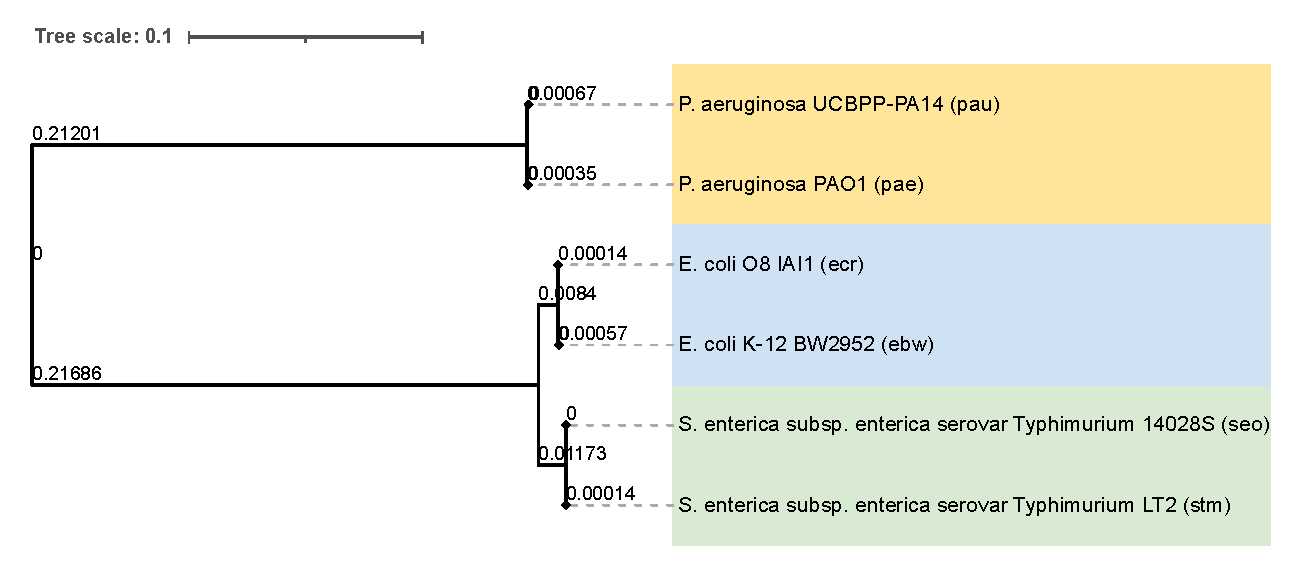
\includegraphics[width=0.5\textwidth,height=\textheight]{"C:/Users/Alex/Google Drive/05-Projects/2020-DDI_networks/figures/Fig1.A.phylogeny.png"} \includegraphics[width=0.5\textwidth,height=\textheight]{"C:/Users/Alex/Google Drive/05-Projects/2020-DDI_networks/figures/Fig1.B.Heatmap1.png"}

Fig. 1. A. Strains phylogeny obtained from HCP concatenated alignments. Branch lengths indicate sequence divergence between strains. B. Heatmap from DDI by strain data. Hierarchical clustering based on euclidean distances was performed for columns and rows. The species clustering accurately matches the species phylogeny. DDI clustering indicates that highly synergistic DDIs (blue squares) are more common in drug combinations that target the same cellular process or that belong to the same chemical class, as can be seen from the accumulation of red lines in the bottom for those categories. C. DDI euclidean distances between strains accumulate as a function of evolutionary time (here shown as phylogenetic distance). This relation can saturate over time as species diverge. Intraspecific comparisons (in blue) have the lowest amount of sequence and chemical divergence, while comparisons with Pseudomonas are the most distant in terms of sequence and chemical divergence. Inset: the same comparison shown as a linear relationship when phylogenetic distance is log transformed. D. Phylomorphospace plot combining DDI data (PCA) with the strains phylogeny. This results in the separation of Pseudomonas and non-Pseudomonas strains along the PC1 axis, which contains almost half of the total variation. PC2 distinguishes between E. coli and S. enterica.

\hypertarget{mapping-drugs-to-their-targets.}{%
\subsection{Mapping drugs to their targets.}\label{mapping-drugs-to-their-targets.}}

Out of the 79 compounds analyzed by Brochado et al.~we were able to identify protein targets for 23 compounds. These compounds had a total of 26 target proteins as identified by their unique protein IDs in E. coli. In addition to this, the most common target category was bacterial penicillin binding protein, a group that refers to targets involved in the biosynthesis of bacterial cell walls. Other categories found, although in a much smaller proportion were ribosomal inhibitors, DNA polymerase inhibitors, topoisomerase inhibitors, thymidylate synthase inhibitors and mitochondrial glycerol-3-phosphate inhibitors (Sup. Table: Drugtargets3\_ecoli.csv). Then, we mapped each of the targets into different biological networks in E. coli by using their Uniprot IDs, and visualized each of the networks using igraph (Sup. Fig. 1). We noticed a great amount of variation across networks, both in number of nodes (2368.727+-1175.486SD) and average path length across networks of (3.859+-0.821SD). In addition, network topology was affected by the type of network under consideration, for example the co-expression (CX) or the high-throughput protein-protein interaction (HT) networks (Sup. Fig. 1). In addition, we calculated the number of targets present in each network, and the number of target inhibitors in each network, obtaining an average of an average of 19.182+- 3.516SD drugs, and 18.545+-6.219SD targets per network (Sup. Table: network\_datatable.csv). These results are not far from the potential maximum of 23 drugs and 29 targets that we identified for this dataset. We also expected some networks to be more biologically relevant than others at expressing the functional relationships between targets, for example the small/medium-scale protein-protein interaction (LC) network (Fig. 2A) would be better suited for the analysis than the co-citation (CC) network (Fig. 2B). This is because it is more difficult to interpret how distance between targets in a citation network depends on the underlying biological interactions, while direct protein-protein interactions are more suited to represent more accurately the functional relationships between target proteins.

Fig. 2. Graphical representations of two biological networks from E. coli, where each node represents a unique Uniprot ID and red nodes are target proteins identified in the analysis. A. Network based on inferred links by small/medium-scale protein-protein interactions (LC). This network contains a smaller number of nodes (767) but the average path length is high relative to other networks (4.8481). B. Network based on inferred links by co-citation of two genes across Pubmed articles for E. coli. This network has a higher number of nodes (2254), but the average path length is smaller (3.6276).

\hypertarget{synergistic-interactions-have-closer-average-distances-in-all-biological-networks-followed-by-additive-and-antagonistic-interactions.}{%
\subsection{Synergistic interactions have closer average distances in all biological networks, followed by additive and antagonistic interactions.}\label{synergistic-interactions-have-closer-average-distances-in-all-biological-networks-followed-by-additive-and-antagonistic-interactions.}}

We measured minimum distance between target proteins across all networks, and observed that synergistic interactions have a smaller average distance between targets across almost all networks, followed by additive and antagonistic interactions. These results were statistically significant for all networks except co-expression (CX) and high-throughput protein-protein interaction (HT) networks (Fig. 3). This result is in agreement with the previously reported observation of synergistic interactions being more common between drugs that target the same cellular process. We performed the same analysis comparing differences in average k edge connectivity between targets (Sup. Fig. 2) and average node degree (Sup. Fig. 3) across networks. However, we didn't find a consistent pattern that showed clear differences between synergistic, additive and antagonistic interactions across all networks, suggesting that there are not clear differences between different types of drug interactions for connectivity or node degree between targets.

Fig. 3. Differences in minimum path length between targets for different types of drug interactions in E. coli for different biological networks. Synergistic interactions have a lower average than additive interactions, followed by antagonisms. This pattern is detected in all networks except the co-expression and the high-throughput protein-protein interaction network.

\hypertarget{clustering-ddis-by-similarity-using-tsne-and-measuring-evolutionary-rates-with-a-multivariate-brownian-motion-model.}{%
\subsection{Clustering DDIs by similarity using tSNE and measuring evolutionary rates with a multivariate brownian motion model.}\label{clustering-ddis-by-similarity-using-tsne-and-measuring-evolutionary-rates-with-a-multivariate-brownian-motion-model.}}

DDIs were clustered by similarity across all species using tSNE. The analysis was repeated for a smaller range of perplexities within this value range and we obtained two possible clustering solutions, one from the large range clustering (Sup. Document 1: tSNE\_plots\_largerange.pdf) and one from the smaller range clustering (Sup. Document 2: tSNE\_plots\_smallrange.pdf). The larger range analysis yielded an optimal clustering solution with 13 distinct clusters at perplexity 703, while the smaller range analysis yielded 4 different clusters returned at perplexity 825 (Fig. 4A). In addition, we mapped the different drug categories and processes targeted into the clustering visualization but we didn't detect any clear patterns showing a clear biological interpretation of the clustering. Next, we conducted 1000 random permutations of the phylo modularity test to determine the optimal clustering solution out of the two obtained. The test supported 13 clusters (p value=0.001, effect size=-26.3594, CR=0.9231, CI=\{0.8643,1.0121\}) over 4 clusters (p value=0.001, effect size=-13.9241, CR=0.985, CI=\{0.9544,1.0049\}), due to the fact that most negative effect sizes have a stronger modular signal (Adams, 2017).

For each of the 13 clusters we calculated multivariate brownian motion evolutionary rates and detected significant differences between clusters (observed rate ratio 12.9955, p value=0.003). Clusters 13 and 2 had very high evolutionary rates with 57.292 and 27.549 respectively, while all the other clusters had rates ranging from 4.409 and 24.184 (Fig 4).

Fig. 4. A. Visualization of tSNE results. Top left: tSNE plot at perplexity 706 yielded 13 unique clusters. Top right: WTT plot showing cluster density and boundaries for perplexity 706. Bottom left: tSNE plot at perplexity 825 yielded 4 clusters. Bottom right. WTT plot showing cluster density and boundaries for perplexity 825. B. Multivariate evolutionary rates for each of the tSNE clusters at perplexity 825 (x axis ordered by rate).

\hypertarget{variation-in-evolutionary-rates-depends-on-several-factors-among-them-the-type-of-interaction-distance-between-target-proteins-and-connectivity.}{%
\subsection{Variation in evolutionary rates depends on several factors, among them the type of interaction, distance between target proteins, and connectivity.}\label{variation-in-evolutionary-rates-depends-on-several-factors-among-them-the-type-of-interaction-distance-between-target-proteins-and-connectivity.}}

We detected significant differences between types of interactions for DDI evolutionary rates, where synergistic interactions have faster evolutionary rates than additive and antagonistic interactions. This pattern was consistently found across all types of biological networks (Fig. 5A). Given the relationship between interaction type and minimum distance we also tested whether evolutionary rates were affected by minimum distance between targets. However, this relationship was not obvious nor consistent across networks, although with some notable exceptions such as the small-medium scale protein-protein interaction network (Fig. 5B) in which there is a decline in evolutionary rates as a function of minimum distance between targets. Other networks such as co-citation (CC),co-functional gene-pairs (GO-BP), or phylogenomic profiles (PG) show a sharp decline in rates as a function of distance followed by an increase in the rate when distance was greater than about 4 steps.

Fig. 5. A. Evolutionary rate as a function of type of interaction and network. Synergistic interactions have higher evolutionary rates than additive and antagonistic interactions across all network types. B. Evolutionary rate as a function of minimum distance between target proteins in the network. It appears that generally the evolutionary rate decreases as a function of distance between targets, however this pattern depends on the network under consideration, having some networks a rebounce for targets connected by more intermediate steps.

We also wanted to evaluate the role that other network parameters play in differences in evolutionary rates for different DDIs, such as connectedness (whether two nodes are connected or not), adjacency (whether two nodes are directly connected or not), k-edge connectivity (the minimum number of connections that have to be broken to disconnect to nodes), and average node degree (the average number of connections in a pair of target proteins). We found that the effect of connectedness and adjacency vary widely by network type. For example, the co-citation (CC), co-expression (CX), co-functional gene pairs (EcoCyc/GO-BP), co-functional gene pairs (GO-BP), EcoliNet integrated networks (EN), high-throughput PPI (HT), genomic context (GN), phylogenetic profiles (PG) and small/medium-scale PPI have slower evolutionary rates in DDI with connected nodes than in disconnected ones (Sup. Fig. 4). Alternatively, we observed that adjacent nodes tend to have higher evolutionary rates than non-adjacent nodes in most types of networks (Sup. Fig. 5), such as co-citation (CC), co-functional gene pairs (EcoCyc), co-functional gene pairs (EcoCyc/GO-BP), co-functional gene pairs (GO-BP), co-occurrence of protein domains (DC), EcoliNet integrated networks (EN) and small/medium-scale protein-protein interactions (LC).

Connectedness between targets was defined using k-edge connectivities different from zero. Differences in evolutionary rates at finer scales, such as modeling evolutionary rates by k-edge connectivity (Sup. Fig. 6) or average node degree between protein targets (Sup. Fig. 7) yielded results that vary widely depending on the type of network and without a straightforward interpretation. In some networks (EcoCyc/GO-BP,EN, GO-BP, HT PPI) it appears that the most connected nodes have higher evolutionary rates, while intermediate and low k-edge connected nodes have a very variable range of evolutionary rates.

\hypertarget{discussion}{%
\section{Discussion}\label{discussion}}

Previous research on network evolution has focused on the study of individual nodes, either by looking at rewiring rates across networks, or by comparing sequence conservation to number of connections per node. Here, we introduce a novel framework to compare evolutionary rates across nodes using network measurements such as minimum distance, connectivity and node degree between proteins. To do so, we explore the relationship between drug drug interactions and network topology that has been previously described in the pharmacological literature (Brochado et al., 2018). DDIs can be connected to specific nodes in the network, if the mode of action for the drug is known. In addition, DDI are quantitative traits that can be compared across species using the phylogenetic comparative method. In this paper, we used a multivariate rate evolutionary model applied to clusters of traits to obtain evolutionary rates of different DDIs. Trait clustering was done due to the limitation in the number of species studied (6 strains of gram negative bacteria). Otherwise, we propose to use a log likelihood test ratio between brownian motion and Ornstein-Uhlenbeck models. This approach however, would require at least 50 strains for robust estimation of the alpha parameter of the Ornstein-Uhlenbeck model. Moreover, this alternative method could be used to determine what role drift and selection play in the evolution of individual DDIs, which can be related to different network measurements as done in this study.

Despite these limitations, our approach produced a general picture of the relationship between different network parameters and evolutionary rates of drug drug interactions. In particular, we showed that the average minimum distance between targets is significantly different in different types of interactions, being smaller in synergistic than additive and antagonistic interactions. This result is in line with the previously known data on synergies being more prevalent in drug combinations that belong to the same chemical class or that target the same cellular process. In addition, we showed that evolutionary rate also depends on the type of interaction, being faster in synergies than in additive and antagonistic interactions. This result was further scrutinized under finer levels of network distance measurements, showing a reduction in rate as a function of minimum distance between targets in most networks. This pattern was unexpected in relation to our original hypothesis, which states that synergistic interactions because they target the same cellular process would be evolutionarily more conserved, since it would be harder to disrupt the fewer edges that exist between the nodes. Alternatively, antagonistic interactions would have a greater flexibility since they target nodes distant from each other in the network, and opportunities for network rewiring would be more common given the higher number of edges between nodes. Our observation however suggests that in fact, the opposite is true, and synergies evolve at a faster rate than antagonism, this may be a result of different factors, such as multi-protein complexes driven by positive selection and network buffering.

Nodes that have a lower distance may have a higher evolutionary rate because they participate in multi-protein complexes, where each connection modulates the formation of novel interactions, or their disruption. Similarly, distance between proteins may affect their rewiring rate, if proteins that are further from each other in the network have less constraints due to having higher changes for rewiring to occur, for example through the elimination of edges between proteins. Alternatively, distance between targets may be inversely related with evolutionary rates, an example of this is if we consider that network buffering plays an important role in evolutionary rates. For example, proteins that are connected by very few steps can be altered easily if the edges break, while proteins that are further apart in the network may have a lower rate of evolution. It is important to also take into account the effect of canalization modulating these effects. For example, the loss of physical interactions between proteins may not mean that their cellular function is compromised, especially if other factors like expression timing and location allow for the process to still be carried out. An example of canalization in networks that takes place in developmental regulation pathways is developmental system drift, which proposes that networks can diverge between species without an evolutionary penalty if the function of the pathway is preserved (True and Haag, 2001). If network canalization effects are dominant network metrics wouldn't affect evolutionary rates significantly. Another possibility is that multi-protein complexes evolve by positive selection because physical interactions between proteins increase the efficiency of metabolic processes. Connections slow down the rate at which proteins evolve, but the connections themselves evolve faster than those of less connected proteins.

\hypertarget{references}{%
\section*{References}\label{references}}
\addcontentsline{toc}{section}{References}

\hypertarget{refs}{}
\leavevmode\hypertarget{ref-Adams2016}{}%
Adams, Dean C, Michael Collyer, Antigoni Kaliontzopoulou, and Emma Sherratt. 2016. ``Geomorph: Software for Geometric Morphometric Analyses.'' Journal Article.

\leavevmode\hypertarget{ref-Armstrong2020}{}%
Armstrong, J. F., E. Faccenda, S. D. Harding, A. J. Pawson, C. Southan, J. L. Sharman, B. Campo, et al. 2020. ``The Iuphar/Bps Guide to Pharmacology in 2020: Extending Immunopharmacology Content and Introducing the Iuphar/Mmv Guide to Malaria Pharmacology.'' Journal Article. \emph{Nucleic Acids Res} 48 (D1): D1006--D1021. \url{https://doi.org/10.1093/nar/gkz951}.

\leavevmode\hypertarget{ref-Brochado2018}{}%
Brochado, A. R., A. Telzerow, J. Bobonis, M. Banzhaf, A. Mateus, J. Selkrig, E. Huth, et al. 2018. ``Species-Specific Activity of Antibacterial Drug Combinations.'' Journal Article. \emph{Nature} 559 (7713): 259--63. \url{https://doi.org/10.1038/s41586-018-0278-9}.

\leavevmode\hypertarget{ref-Cork2004}{}%
Cork, J. M., and M. D. Purugganan. 2004. ``The Evolution of Molecular Genetic Pathways and Networks.'' Journal Article. \emph{Bioessays} 26 (5): 479--84. \url{https://doi.org/10.1002/bies.20026}.

\leavevmode\hypertarget{ref-Cowen2008}{}%
Cowen, L. E., and W. J. Steinbach. 2008. ``Stress, Drugs, and Evolution: The Role of Cellular Signaling in Fungal Drug Resistance.'' Journal Article. \emph{Eukaryot Cell} 7 (5): 747--64. \url{https://doi.org/10.1128/EC.00041-08}.

\leavevmode\hypertarget{ref-Csardi2016}{}%
Csardi, Gabor, and Tamas Nepusz. 2006. ``The Igraph Software Package for Complex Network Research.'' Journal Article. \emph{InterJournal, Complex Systems} 1695 (5): 1--9.

\leavevmode\hypertarget{ref-Cusick2005}{}%
Cusick, M. E., N. Klitgord, M. Vidal, and D. E. Hill. 2005. ``Interactome: Gateway into Systems Biology.'' Journal Article. \emph{Hum Mol Genet} 14 Spec No. 2: R171--81. \url{https://doi.org/10.1093/hmg/ddi335}.

\leavevmode\hypertarget{ref-Fang2019}{}%
Fang, Y., C. Liu, J. Lin, X. Li, K. N. Alavian, Y. Yang, and Y. Niu. 2019. ``PhySpeTree: An Automated Pipeline for Reconstructing Phylogenetic Species Trees.'' Journal Article. \emph{BMC Evol Biol} 19 (1): 219. \url{https://doi.org/10.1186/s12862-019-1541-x}.

\leavevmode\hypertarget{ref-Fraser2002}{}%
Fraser, H. B., A. E. Hirsh, L. M. Steinmetz, C. Scharfe, and M. W. Feldman. 2002. ``Evolutionary Rate in the Protein Interaction Network.'' Journal Article. \emph{Science} 296 (5568): 750--2. \url{https://doi.org/10.1126/science.1068696}.

\leavevmode\hypertarget{ref-Garriga2018}{}%
Garriga, Joan, and Frederic Bartumeus. 2018. ``BigMap: Big Data Mapping with Parallelized T-Sne.'' Journal Article. \emph{arXiv Preprint arXiv:1812.09869}.

\leavevmode\hypertarget{ref-Ghadie2018}{}%
Ghadie, M. A., J. Coulombe-Huntington, and Y. Xia. 2018. ``Interactome Evolution: Insights from Genome-Wide Analyses of Protein-Protein Interactions.'' Journal Article. \emph{Curr Opin Struct Biol} 50: 42--48. \url{https://doi.org/10.1016/j.sbi.2017.10.012}.

\leavevmode\hypertarget{ref-Hadicke2017}{}%
Hädicke, Oliver, and Steffen Klamt. 2017. ``EColiCore2: A Reference Network Model of the Central Metabolism of Escherichia Coli and Relationships to Its Genome-Scale Parent Model.'' Journal Article. \emph{Scientific Reports} 7 (1): 1--15.

\leavevmode\hypertarget{ref-Jensen1976}{}%
Jensen, R. A. 1976. ``Enzyme Recruitment in Evolution of New Function.'' Journal Article. \emph{Annu Rev Microbiol} 30 (1): 409--25. \url{https://doi.org/10.1146/annurev.mi.30.100176.002205}.

\leavevmode\hypertarget{ref-Jin2013}{}%
Jin, Y., D. Turaev, T. Weinmaier, T. Rattei, and H. A. Makse. 2013. ``The Evolutionary Dynamics of Protein-Protein Interaction Networks Inferred from the Reconstruction of Ancient Networks.'' Journal Article. \emph{PLoS One} 8 (3): e58134. \url{https://doi.org/10.1371/journal.pone.0058134}.

\leavevmode\hypertarget{ref-Kane2013}{}%
Kane, Michael, John W Emerson, and Stephen Weston. 2013. ``Scalable Strategies for Computing with Massive Data.'' Journal Article. \emph{Journal of Statistical Software} 55 (1): 1--19.

\leavevmode\hypertarget{ref-Kanehisa2000}{}%
Kanehisa, M., and S. Goto. 2000. ``KEGG: Kyoto Encyclopedia of Genes and Genomes.'' Journal Article. \emph{Nucleic Acids Res} 28 (1): 27--30. \url{https://doi.org/10.1093/nar/28.1.27}.

\leavevmode\hypertarget{ref-Kim2015}{}%
Kim, H., J. E. Shim, J. Shin, and I. Lee. 2015. ``EcoliNet: A Database of Cofunctional Gene Network for Escherichia Coli.'' Journal Article. \emph{Database (Oxford)} 2015. \url{https://doi.org/10.1093/database/bav001}.

\leavevmode\hypertarget{ref-Lehar2007}{}%
Lehar, J., G. R. Zimmermann, A. S. Krueger, R. A. Molnar, J. T. Ledell, A. M. Heilbut, 3rd Short G. F., et al. 2007. ``Chemical Combination Effects Predict Connectivity in Biological Systems.'' Journal Article. \emph{Mol Syst Biol} 3 (1): 80. \url{https://doi.org/10.1038/msb4100116}.

\leavevmode\hypertarget{ref-Nguyen2015}{}%
Nguyen, L. T., H. A. Schmidt, A. von Haeseler, and B. Q. Minh. 2015. ``IQ-Tree: A Fast and Effective Stochastic Algorithm for Estimating Maximum-Likelihood Phylogenies.'' Journal Article. \emph{Mol Biol Evol} 32 (1): 268--74. \url{https://doi.org/10.1093/molbev/msu300}.

\leavevmode\hypertarget{ref-Picard2008}{}%
Picard, F., J. J. Daudin, M. Koskas, S. Schbath, and S. Robin. 2008. ``Assessing the Exceptionality of Network Motifs.'' Journal Article. \emph{J Comput Biol} 15 (1): 1--20. \url{https://doi.org/10.1089/cmb.2007.0137}.

\leavevmode\hypertarget{ref-Robbins2015}{}%
Robbins, N., M. Spitzer, T. Yu, R. P. Cerone, A. K. Averette, Y. S. Bahn, J. Heitman, D. C. Sheppard, M. Tyers, and G. D. Wright. 2015. ``An Antifungal Combination Matrix Identifies a Rich Pool of Adjuvant Molecules That Enhance Drug Activity Against Diverse Fungal Pathogens.'' Journal Article. \emph{Cell Rep} 13 (7): 1481--92. \url{https://doi.org/10.1016/j.celrep.2015.10.018}.

\leavevmode\hypertarget{ref-Shou2011}{}%
Shou, C., N. Bhardwaj, H. Y. Lam, K. K. Yan, P. M. Kim, M. Snyder, and M. B. Gerstein. 2011. ``Measuring the Evolutionary Rewiring of Biological Networks.'' Journal Article. \emph{PLoS Comput Biol} 7 (1): e1001050. \url{https://doi.org/10.1371/journal.pcbi.1001050}.

\leavevmode\hypertarget{ref-Spitzer2011}{}%
Spitzer, M., E. Griffiths, K. M. Blakely, J. Wildenhain, L. Ejim, L. Rossi, G. De Pascale, et al. 2011. ``Cross-Species Discovery of Syncretic Drug Combinations That Potentiate the Antifungal Fluconazole.'' Journal Article. \emph{Mol Syst Biol} 7: 499. \url{https://doi.org/10.1038/msb.2011.31}.

\leavevmode\hypertarget{ref-Szocs2020}{}%
Szöcs, Eduard, Tamás Stirling, Eric R Scott, Andreas Scharmüller, and Ralf B Schäfer. 2020. ``Webchem: An R Package to Retrieve Chemical Information from the Web.'' Journal Article. \emph{Journal of Statistical Software} 93 (1): 1--17.

\leavevmode\hypertarget{ref-Wagner2003}{}%
Wagner, Andreas. 2003. ``How the Global Structure of Protein Interaction Networks Evolves.'' Journal Article. \emph{Proceedings of the Royal Society of London. Series B: Biological Sciences} 270 (1514): 457--66. \url{https://www.ncbi.nlm.nih.gov/pmc/articles/PMC1691265/pdf/12641899.pdf}.

\leavevmode\hypertarget{ref-Yeh2009}{}%
Yeh, P. J., M. J. Hegreness, A. P. Aiden, and R. Kishony. 2009. ``Drug Interactions and the Evolution of Antibiotic Resistance.'' Journal Article. \emph{Nat Rev Microbiol} 7 (6): 460--6. \url{https://doi.org/10.1038/nrmicro2133}.

\leavevmode\hypertarget{ref-Zotenko2008}{}%
Zotenko, Elena, Julian Mestre, Dianne P O'Leary, and Teresa M Przytycka. 2008. ``Why Do Hubs in the Yeast Protein Interaction Network Tend to Be Essential: Reexamining the Connection Between the Network Topology and Essentiality.'' Journal Article. \emph{PLoS Computational Biology} 4 (8): e1000140.


\end{document}

